% !TEX program = xelatex
% !BIB program = bibtex

\documentclass[11pt,a4paper]{article}
\usepackage[UTF8]{ctex}
\usepackage{float}
\usepackage{amsmath}
\usepackage{amsfonts}
\usepackage{enumerate}
\usepackage{booktabs}
\usepackage{graphicx}
\usepackage{longtable}
\usepackage{subfigure}
\usepackage{multirow}
\usepackage{url}

% for reference 
\usepackage{hyperref}
\usepackage{cleveref}
\crefname{equation}{式}{式}
\Crefname{equation}{式}{式}
\crefname{table}{表}{表}
\Crefname{table}{表}{表}
\crefname{figure}{图}{图}
\Crefname{figure}{图}{图}

% Microsoft Word A4 paper default layout 
\usepackage[a4paper, left=2cm, right=2cm, top=2cm, bottom=2cm]{geometry}

\title{媒体计算实验一\\基于GraphCut的纹理合成}
\author{2017011620 \quad 计73 \quad 李家昊}
\date{\today}

\begin{document}

\maketitle

\section{工作内容}

本次实验中,我基于GraphCut算法实现了纹理合成\cite{kwatra2003graphcut},实现了基本的块切割算法和三种偏移生成算法,扩展的切割算法改进,偏移算法加速,以及影像拼接。

\section{块切割算法}

当一张新图(patch)覆盖在原有的纹理图(texture)上时,需要在它们的重叠部分进行切割,使得两图之间过渡自然,割缝区域尽可能与图片结构保持一致。我们可以采用GraphCut算法,首先构建出以像素为节点的图,然后求出图的最小割,最后进行块的像素拷贝,如\Cref{fig:graphcut}。

\begin{figure}[H]
    \centering
    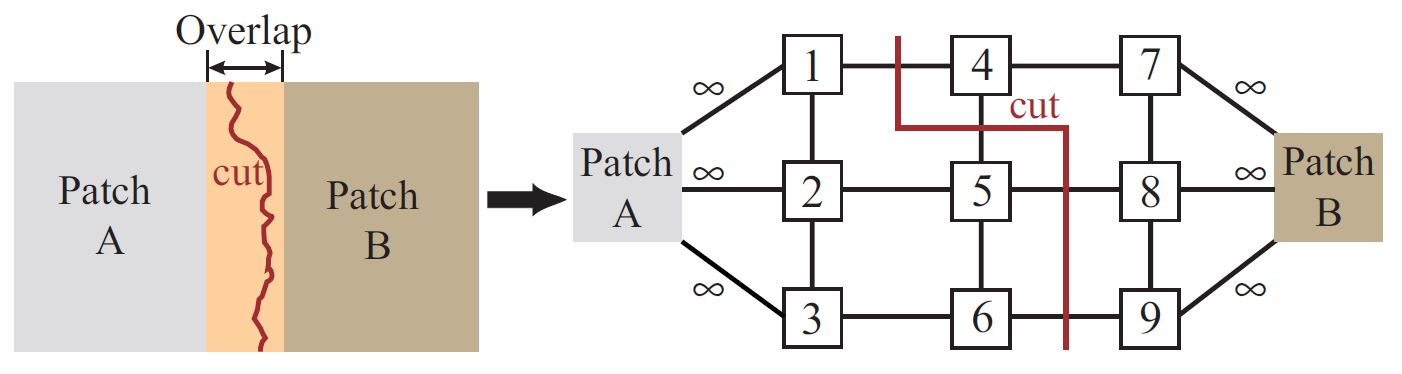
\includegraphics[width=0.7\textwidth]{fig/graphcut.jpg}
    \caption{基于GraphCut的块切割算法}
    \label{fig:graphcut}
\end{figure}

\paragraph{建图} 将重叠部分的每个像素视作一个图节点,相邻像素之间连一条边,边的容量为这两个像素在patch和texture中的色差和,即,
\begin{equation}\label{eq:energy}
    M(a,b,\mathbf{A},\mathbf{B}) = ||\mathbf{A}(a)-\mathbf{B}(a)|| + ||\mathbf{A}(b)-\mathbf{B}(b)||
\end{equation}

其中$a,b$为两个像素的位置,$\mathbf{A}$表示texture,$\mathbf{B}$表示patch。同时,令patch边界的像素通过$\infty$边连接到超级源$s$,texture边界的像素通过$\infty$边连接到超级汇$t$,这样就组成了一个网络流图$G$。

这样建图以后,如果两个相邻位置$a,b$在patch和texture上的像素都越相近,其连边的容量越小,则越容易被最小割算法切割开,最终使得$\mathbf{A}(a)$与$\mathbf{B}(b)$相邻,但由于$\mathbf{A}(a)$与$\mathbf{B}(a)$相近,$\mathbf{B}(b)$与$\mathbf{A}(b)$相近,因此切割后割缝两旁的差异较小。

\paragraph{求出最小割} 对于网络流图$G$,可以通过最高标号预留推进算法(Highest-Label Preflow-Push)\cite{cheriyan1989analysis}求出其最小s-t割。

\paragraph{块的像素拷贝} 得到最小s-t割后,将重叠区域与patch相连的割集拷贝到texture,并且将非重叠部分的patch部分拷贝到texture,这样就完成了块切割。

在给定的键盘纹理上手动指定patch的放置位置,实验结果如\Cref{fig:blockcut}。可以看出,GraphCut算法取得了不错的效果,前两排按键得到了很好的扩展,由于最下面的S键左边是空格键,因此不能完整的融合。

\begin{figure}[H]
    \centering
    \subfigure[原始纹理]{
        
\includegraphics[height=3.2cm]{../data/keyboard.jpg}
    }
    \subfigure[叠加patch后进行块切割]{
        
\includegraphics[height=3.2cm]{../output/blockcut.png}
    }
    \caption{块切割效果}
    \label{fig:blockcut}
\end{figure}

\section{三种块偏移生成算法}

块偏移位置对块切割算法的效果有决定性影响,上面情况中,我通过手动指定patch偏移位置,然后进行块切割,但实际情况中,算法需要自动选择patch的偏移位置,并进行块切割。下面实现了三种偏移生成算法:随机生成,整块匹配算法,子块匹配算法。其中随机生成和整块匹配算法用于patch填充,子块匹配算法用于最终refine。

\paragraph{随机生成(Random placement)} 在随机生成算法中,我们首先求出texture中第一个未被覆盖的像素$(x,y)$,记patch的大小为$w\times h$,则我们在$[x-w/4,x+w/4) \times [y-h/4,y+h/4)$区间内随机选取patch的中心位置$(x_c,y_c)$,进行块切割。随机生成方法效率非常高,在非结构性纹理上效果不错,实验结果如\Cref{fig:fill_patch}。

\paragraph{整块匹配(Entire patch matching)} 对于结构性纹理,需要采用整块匹配的方法寻找最优偏移。具体来说,我们遍历每个可能的patch偏移$t$,计算此时patch与texture在重叠部分的均方误差$C(t)$(论文中称为SSD,sum-of-squared-differences),即,
\begin{equation}\label{eq:entire_patch}
    C(t) = \frac{1}{|\mathbf{A}_t|}\sum_{p\in\mathbf{A}_t}|\mathbf{I}(p)-\mathbf{O}(p+t)|^2
\end{equation}

其中$\mathbf{I}$为patch,$\mathbf{O}$为texture,$\mathbf{A}_t$为patch和texture的重叠部分。偏移对应的$C(t)$越小,其选取的概率$P$则越大,满足以下关系,
\begin{equation}
    P(t) \propto \exp\left(-\frac{C(t)}{k\sigma^2}\right)
\end{equation}

在具体实现中,我发现依概率选取偏移将导致算法不稳定,因此我直接选取了$C(t)$最小的偏移,实验结果如\Cref{fig:fill_patch}。

\begin{figure}[H]
    \centering
    \subfigure[原始纹理]{
        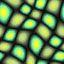
\includegraphics[height=2cm]{../data/green.jpg}
    }
    \subfigure[随机偏移]{
        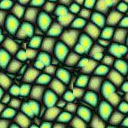
\includegraphics[height=4cm]{../output/random_green.png}
    }
    \subfigure[整块匹配]{
        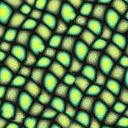
\includegraphics[height=4cm]{../output/entire_green.png}
    }

    \subfigure[原始纹理]{
        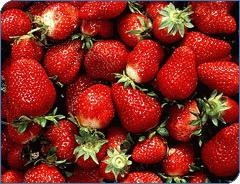
\includegraphics[height=2cm]{../data/strawberry.jpg}
    }
    \subfigure[随机偏移]{
        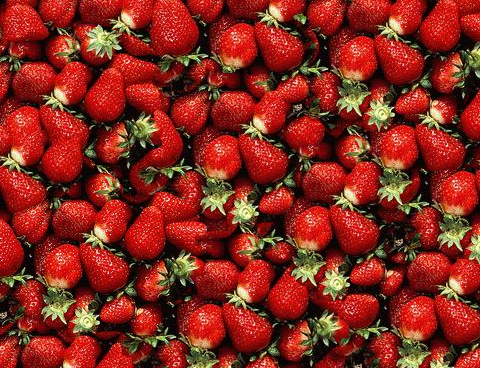
\includegraphics[height=4cm]{../output/random_strawberry.png}
    }
    \subfigure[整块匹配]{
        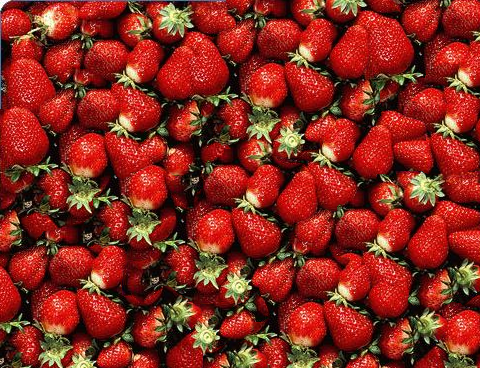
\includegraphics[height=4cm]{../output/entire_strawberry.png}
    }

    \subfigure[原始纹理]{
        
\includegraphics[height=2cm]{../data/keyboard.jpg}
    }
    \subfigure[随机偏移]{
        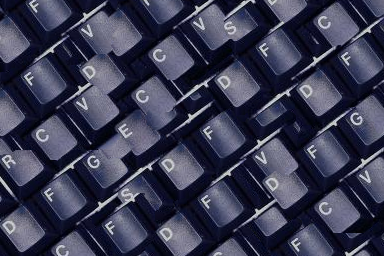
\includegraphics[height=4cm]{../output/random_keyboard.png}
    }
    \subfigure[整块匹配]{
        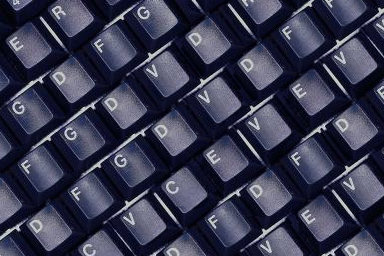
\includegraphics[height=4cm]{../output/entire_keyboard.png}
    }
    \caption{随机偏移与整块匹配的效果对比}
    \label{fig:fill_patch}
\end{figure}

\paragraph{子块匹配(Sub-patch matching)} 子块匹配算法仅用于最终的refine。当texture完全被patch填满后,我们希望优化其中代价比较大的割缝,首先在texture中找到切割代价最大的矩形子块(error-region),记其大小为$w_e \times h_e$,记像素$(x,y)$的左方和上方的切割代价和为$Q(x,y)$(未被切割则为0),则以$(x,y)$为左上角的子块的总代价为,
\begin{equation}
    E(x,y) = (Q * F)(x,y)
\end{equation}

其中$F \in \mathbb{R}^{w_e \times h_e}$为全1矩阵,卷积可以利用FFT加速计算。我们找到$E(x,y)$最小时对应的坐标$(x_e,y_e)$,就得到了代价最大的子块,记为$\mathbf{S}_{\mathbf{O}}=[x_e,x_e+w_e) \times [y_e,y_e+h_e)$。

我们希望新patch能够完全覆盖该texture子块,因此子块的大小应当小于patch的大小,我们遍历texture子块在patch中所有可能的偏移,计算该texture子块与patch的SSD代价,
\begin{equation}\label{eq:sub_patch}
    C(t) = \sum_{p\in \mathbf{S}_{\mathbf{O}}}|\mathbf{I}(p-t)-\mathbf{O}(p)|^2
\end{equation}

其中$\mathbf{S}_{\mathbf{O}}$表示texture矩形子块,$\mathbf{I}$表示patch,$\mathbf{O}$表示texture。

子块匹配算法通常与旧割更新算法配合使用,在最终refine时,我们采用子块匹配算法求出代价最大的子块,以及可以覆盖子块的最佳patch偏移,如\Cref{fig:refine_steps},可以看出,代价最大的子块通常在割缝结合处附近,子块内的割缝均被新割更新,从而降低切割代价。

\begin{figure}[H]
    \centering
    \subfigure[Refine Step 0]{
        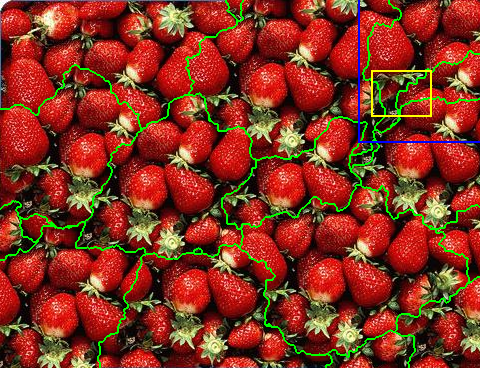
\includegraphics[width=0.4\textwidth]{../output/refine0.png}
    }
    \subfigure[Refine Step 1]{
        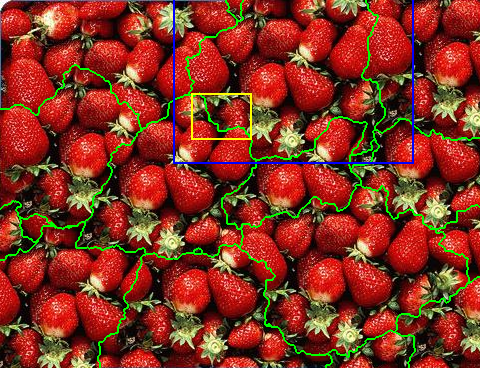
\includegraphics[width=0.4\textwidth]{../output/refine1.png}
    }
    \subfigure[Refine Step 2]{
        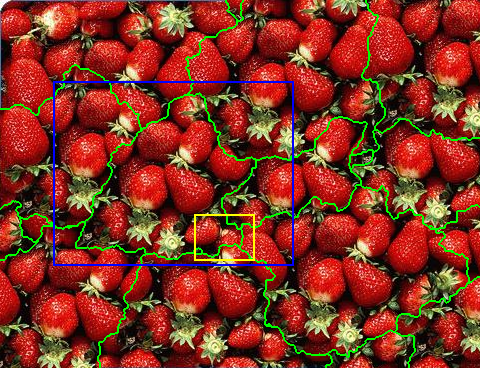
\includegraphics[width=0.4\textwidth]{../output/refine2.png}
    }
    \subfigure[Refine Step 3]{
        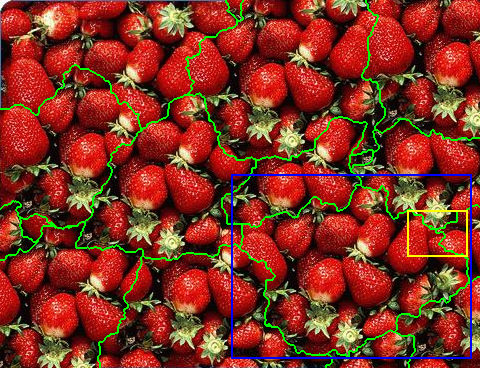
\includegraphics[width=0.4\textwidth]{../output/refine3.png}
    }
    \caption{Refine过程,图中绿线代表割缝,黄框表示代价最大的子块,蓝框表示最佳patch偏移}
    \label{fig:refine_steps}
\end{figure}

\section{切割算法改进}

\subsection{考虑Old Cuts}

当patch与texture的重叠区域内存在先前的切割时,我们可以用新割更新旧割,降低总切割代价。如\Cref{fig:oldcut},记$\mathbf{A}_s$为节点$s$拷贝到texture时对应的patch,记当前的patch为$\mathbf{B}$,如果在两个像素之间存在旧割,例如节点1和4,则在节点1,4之间插入一个切割节点$S_1$(seam node),$S_1$与$\mathbf{B}$和节点1,4均有连边,$S_1$与$\mathbf{B}$的连边容量为先前的$M(1,4,\mathbf{A}_1,\mathbf{A}_4)$(如果割断则将维持旧割),与节点1的连边容量为$M(1,4,\mathbf{A}_1,\mathbf{B})$(如果割断则节点4将被$\mathbf{B}$覆盖),与节点4的连边容量为$M(1,4,\mathbf{B},\mathbf{A}_4)$(如果割断则节点1将被$\mathbf{B}$覆盖),这样就得到了一个改进的网络流图$G$,接下来按照相同的流程,求出$G$的最小割,再进行块的像素拷贝即可。

\begin{figure}[H]
    \centering
    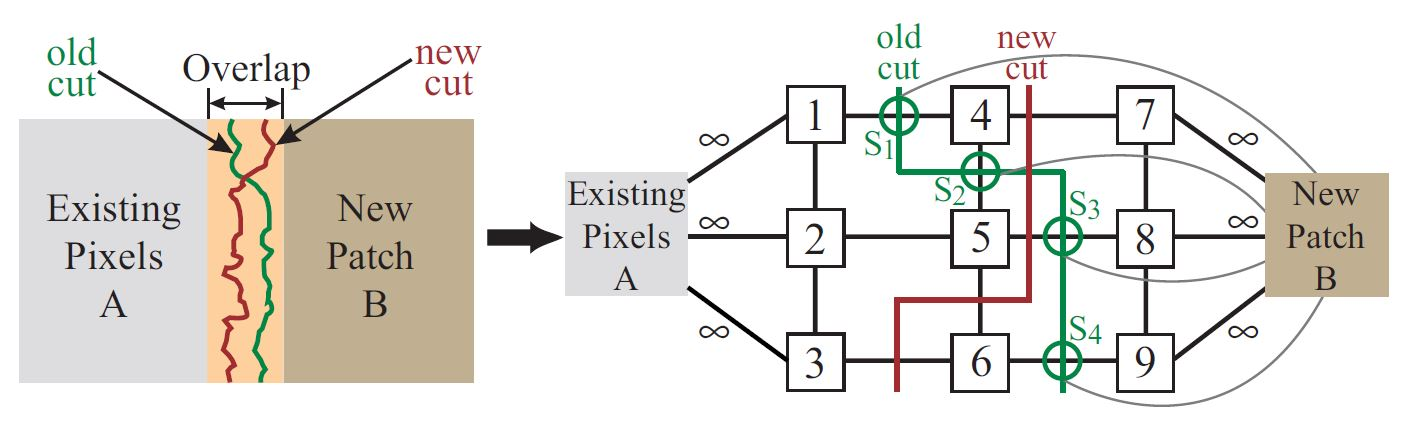
\includegraphics[width=0.7\textwidth]{fig/update_cut.jpg}
    \caption{建图时引入旧割}
    \label{fig:oldcut}
\end{figure}

更新旧割的效果如\Cref{fig:update_cut},可以看出,新割在旧割的交汇处进行了图像的覆盖,使得图片过渡更加自然。更多实验结果详见\Cref{fig:refine_steps}。

\begin{figure}[H]
    \centering
    \subfigure[Old Cuts]{
        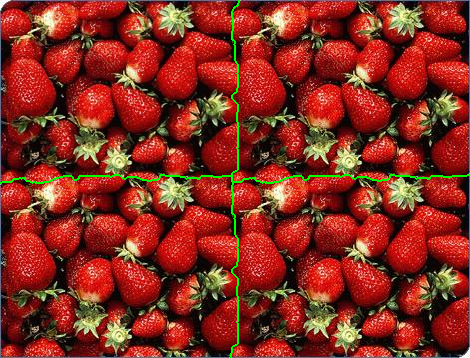
\includegraphics[width=0.4\textwidth]{../output/oldcut.png}
    }
    \subfigure[Net Cuts]{
        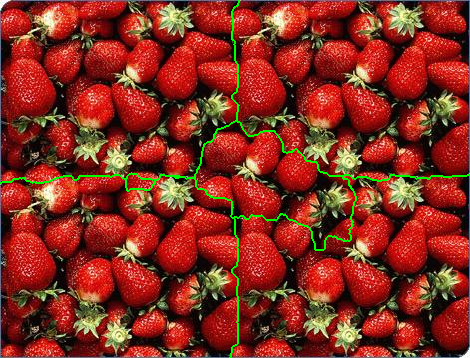
\includegraphics[width=0.4\textwidth]{../output/newcut.png}
    }
    \caption{旧割的更新}
    \label{fig:update_cut}
\end{figure}

\subsection{处理Surrounded Regions}

当patch完全重叠在texture的已填充区域时,如果未考虑旧割,将不会有任何像素节点连接到超级源$s$,此时可以在重叠区域中强制将一个像素节点连接到超级源$s$;但由于我考虑了旧割,因此只要重叠区域内有旧割,必然有边连接到超级源$s$,那么可以按之前的流程相同处理,效果如\Cref{fig:update_cut},这里不再赘述,如果没有旧割,说明重叠部分是一张完整的patch,此时也没有更新的必要。

\subsection{能量函数引入梯度信息}

在\Cref{eq:energy}中,我们只考虑了两张图在两点的色差,而未考虑图片本身的梯度,图片梯度大的时候应当容许的误差更大,因此可以将梯度作为归一化因子,即,
\begin{equation}
    M'(a,b,\mathbf{A},\mathbf{B}) = \frac{M(a,b,\mathbf{A},\mathbf{B})}{||\mathbf{G}_\mathbf{A}^d(a)||+||\mathbf{G}_\mathbf{A}^d(b)||+||\mathbf{G}_\mathbf{B}^d(a)||+||\mathbf{G}_\mathbf{B}^d(b)||}
\end{equation}

其中$d$为$a,b$像素的方向(水平/垂直),$\mathbf{G}_\mathbf{A}^d(a)$为$\mathbf{A}$图在$a$点处$d$方向上的梯度。梯度信息对图像拼接有较大的正向作用,在普通的纹理合成上影响不大,甚至有负面效果,实验结果如\Cref{fig:grad}。

\begin{figure}[H]
    \centering
    \subfigure{
        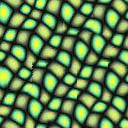
\includegraphics[height=4cm]{../output/grad_green.png}
    }
    \subfigure{
        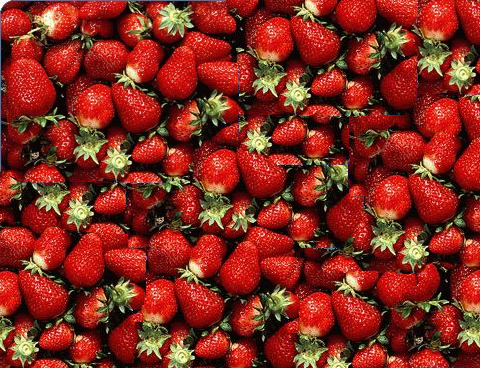
\includegraphics[height=4cm]{../output/grad_strawberry.png}
    }
    \subfigure{
        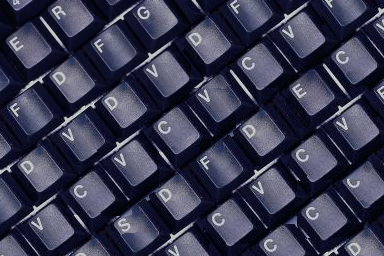
\includegraphics[height=4cm]{../output/grad_keyboard.png}
    }
    \caption{引入梯度信息后的纹理合成效果}
    \label{fig:grad}
\end{figure}

\section{偏移算法加速}

在\Cref{eq:entire_patch}和\Cref{eq:sub_patch}中,记像素数量为$n$,偏移$t$需要遍历$O(n)$个取值,对于每个固定的$t$,计算$C(t)$需要做$O(n)$次乘法和加法,因此算法的时间复杂度为$O(n^2)$,可以进一步优化。

对于子块匹配,展开\Cref{eq:sub_patch}得到,
\begin{equation}
    C(t) = \sum_p\mathbf{I}^2(p-t) + \sum_p\mathbf{O}^2(p) - 2\sum_p\mathbf{I}(p-t)\mathbf{O}(p)
\end{equation}

可以一次计算所有的$C(t)$,平方项$\sum_p\mathbf{I}^2(p-t)$和$\sum_p\mathbf{O}^2(p)$可通过前缀和在$O(n)$时间内计算得到,交叉项$\sum_p\mathbf{I}(p-t)\mathbf{O}(p)=(\mathbf{I}*\mathbf{O})(t)$,卷积可通过FFT在$O(n\log n)$时间内计算得到。

更一般的,对于整块匹配,记texture已填充区域的掩膜为$\mathbf{A}_{\mathbf{O}}$,patch的掩膜为全1矩阵$\mathbf{A}_\mathbf{I}$,展开\Cref{eq:entire_patch}得到,
\begin{equation}
    C(t) = \frac{\mathbf{I}^2 * \mathbf{A}_\mathbf{O} + \mathbf{O}^2 * \mathbf{A}_\mathbf{I} - 2\cdot\mathbf{I}*\mathbf{O}}{\mathbf{A}_\mathbf{I} * \mathbf{A}_\mathbf{O}}(t)
\end{equation}

卷积可通过FFT加速到$O(n \log n)$时间,算法的总时间复杂度同样为$O(n \log n)$。

\begin{table}[H]
    \centering
    \caption{整块匹配加速前后的运行时间}
    \label{tab:entire_speed}
    \begin{longtable}{l|ccc}
        \toprule
         & 加速前全局搜索 & 加速前局部搜索 & FFT\tabularnewline
        \midrule
        % \endhead
        运行时间(s) & 19.64 & 3.71 & \textbf{0.14}\tabularnewline
        \bottomrule
    \end{longtable}
\end{table}

经过FFT加速后,整块匹配和子块匹配算法选取的偏移均与原来一致,块切割纹理合成效果也相同,加速前后的运行时间如\Cref{tab:entire_speed},可以看出,经过FFT加速后,算法的执行效率有了很大的提升。

\section{影像拼接}

给定多张不同角度拍摄的照片,照片之间有重叠部分,我们需要将它们拼接成一张全景图,拼接过程分为三步:图像对齐,GraphCut,泊松融合。

\paragraph{图像对齐} 我们需要将这些图像对齐到同一视角下,记给定的$n$张图像为$\{\mathbf{I}_i\}_{i=1}^n$,通过SIFT\cite{lowe1999object}特征点匹配,可求得相邻两张图片$\mathbf{I}_{i}$到$\mathbf{I}_{i-1}$的单应性矩阵为$\{\mathbf{H}_{i,i-1}\}_{i=1}^{n}$,这里规定$\mathbf{H}_{1,0}$为单位阵,则$\mathbf{I}_k$到$\mathbf{I}_1$的单应性矩阵为,
\begin{equation}
    \mathbf{H}_{k,1} = \prod_{i=1}^k \mathbf{H}_{i,i-1}
\end{equation}

对每张图片$\mathbf{I}_k$,我们根据单应性矩阵$\mathbf{H}_{k,1}$进行透视变换,将它对齐到第一张图,实验结果如\Cref{fig:campus_align}。

\begin{figure}[H]
    \centering
    \subfigure[原始A图]{
        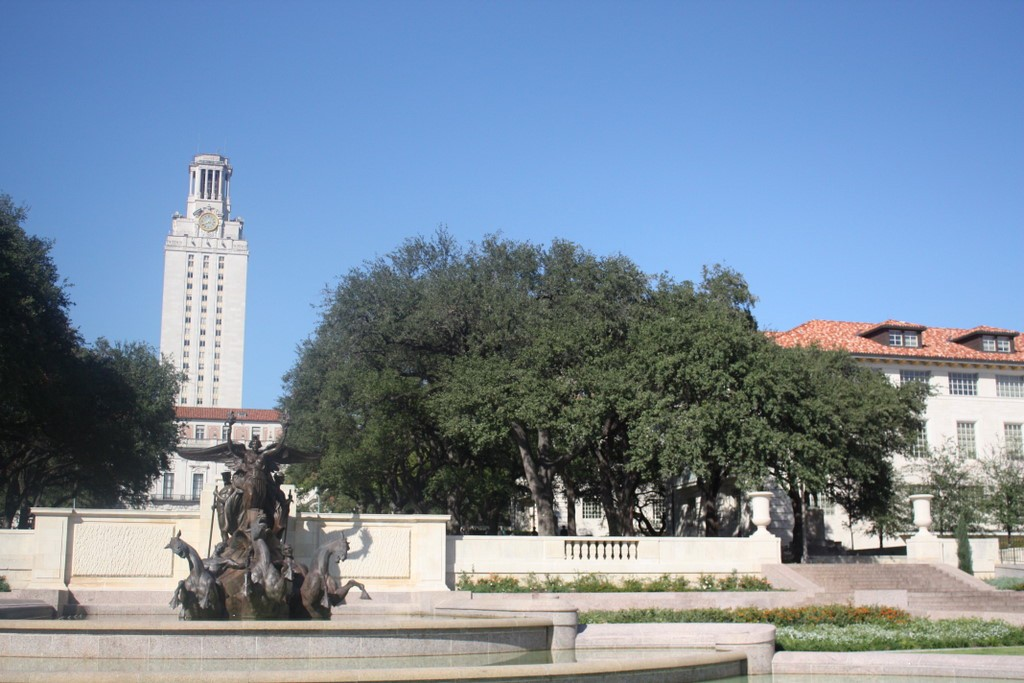
\includegraphics[width=0.45\textwidth]{../data/campus/00.jpg}
    }
    \subfigure[原始B图]{
        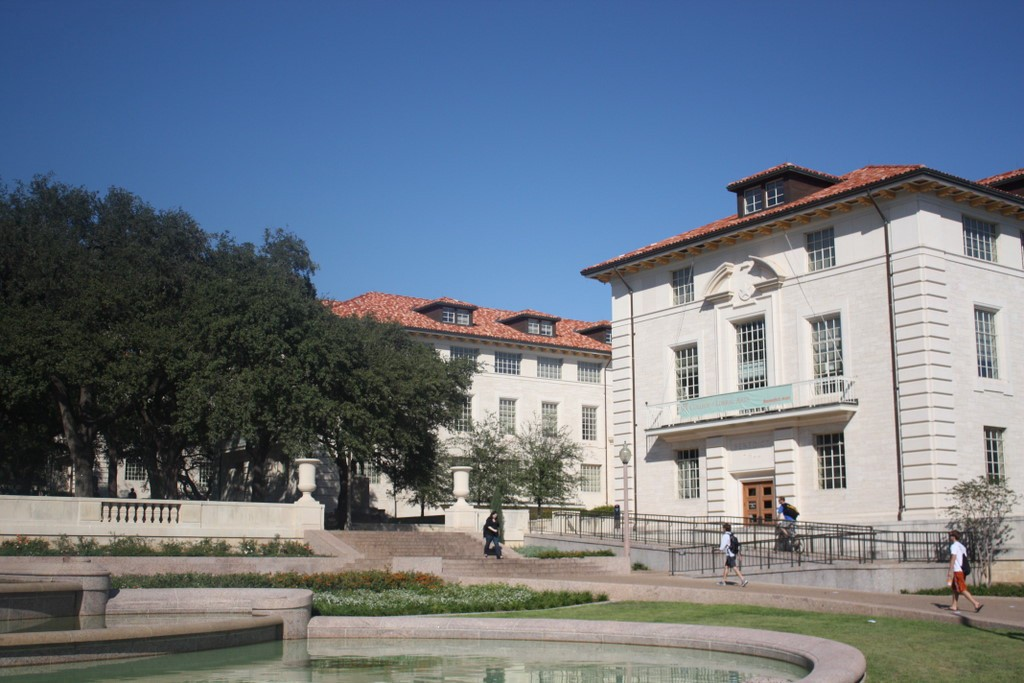
\includegraphics[width=0.45\textwidth]{../data/campus/01.jpg}
    }
    \subfigure[对齐A图]{
        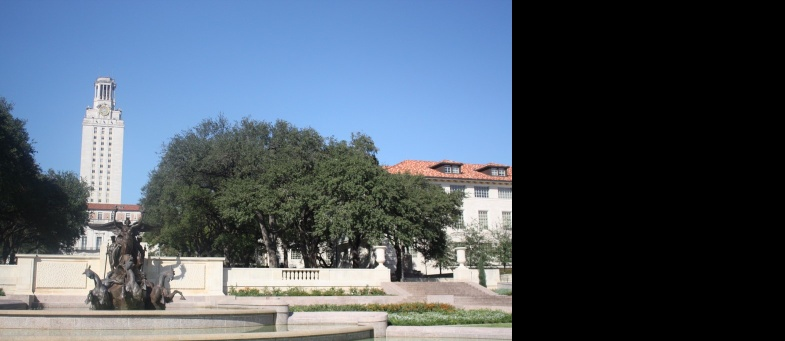
\includegraphics[width=0.45\textwidth]{../output/campus_align/00.jpg}
    }
    \subfigure[对齐B图]{
        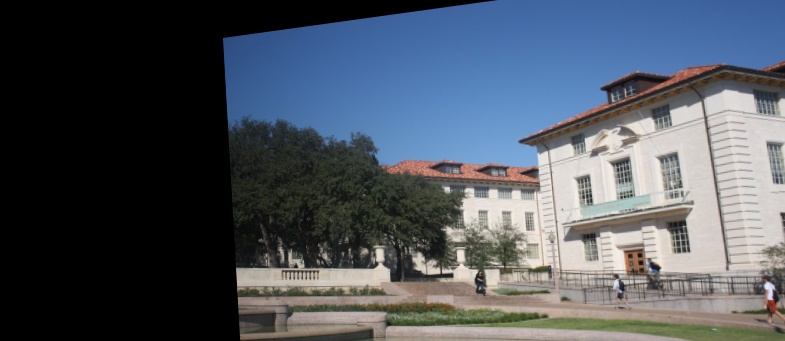
\includegraphics[width=0.45\textwidth]{../output/campus_align/01.jpg}
    }
    \caption{对齐效果}
    \label{fig:campus_align}
\end{figure}

\paragraph{GraphCut} 得到对齐且有重合部分的图像后,我们将一张图作为texture,另一张图作为patch,偏移量为零(已对齐),对两者重叠部分做GraphCut,得到一个最小割,结果如\Cref{fig:campus_graphcut}。

\begin{figure}[H]
    \centering
    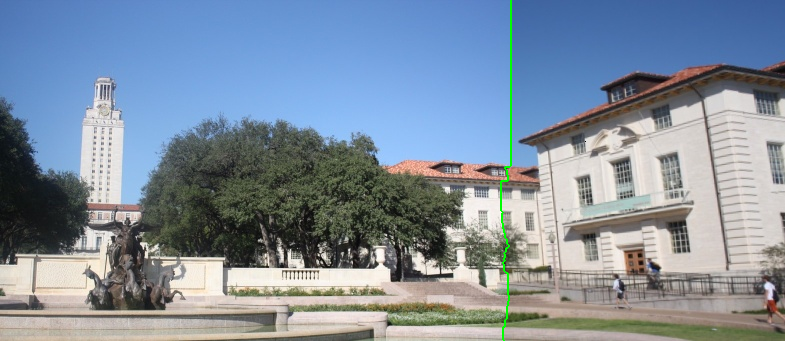
\includegraphics[width=0.8\textwidth]{../output/campus_graphcut.png}
    \caption{GraphCut效果}
    \label{fig:campus_graphcut}
\end{figure}

\paragraph{泊松融合} 得到最小割后,我们对图像进行泊松融合\cite{perez2003poisson},在最小割上加入边界约束,最终结果如\Cref{fig:campus_poisson}。

\begin{figure}[H]
    \centering
    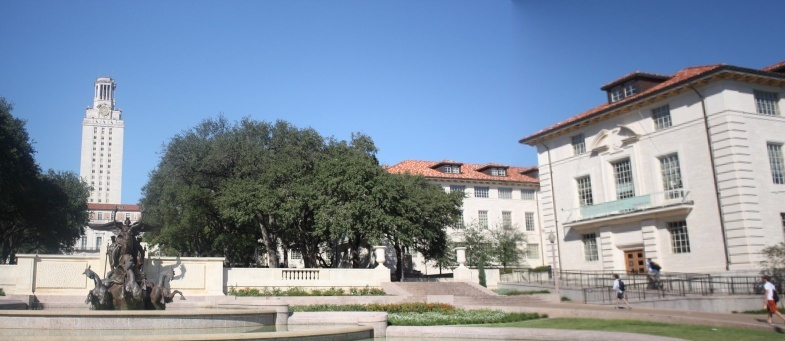
\includegraphics[width=0.8\textwidth]{../output/campus_poisson.jpg}
    \caption{最终效果}
    \label{fig:campus_poisson}
\end{figure}

\paragraph{更多结果} 在Adobe Panoramas Dataset上有很多影像拼接的数据,这里选取了一组金门大桥的图片作为测试,原始图片如\Cref{fig:golden_org},对齐后照片如\Cref{fig:golden_align},GraphCut和泊松融合后得到最终结果如\Cref{fig:golden_poisson}。

\begin{figure}[H]
    \centering
    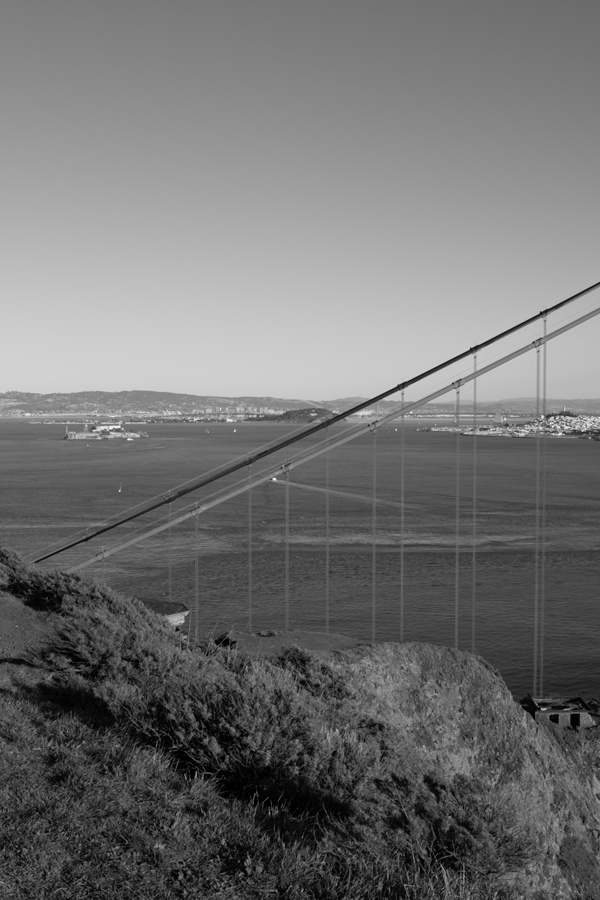
\includegraphics[width=0.16\textwidth]{../data/goldengate/00.jpg}
    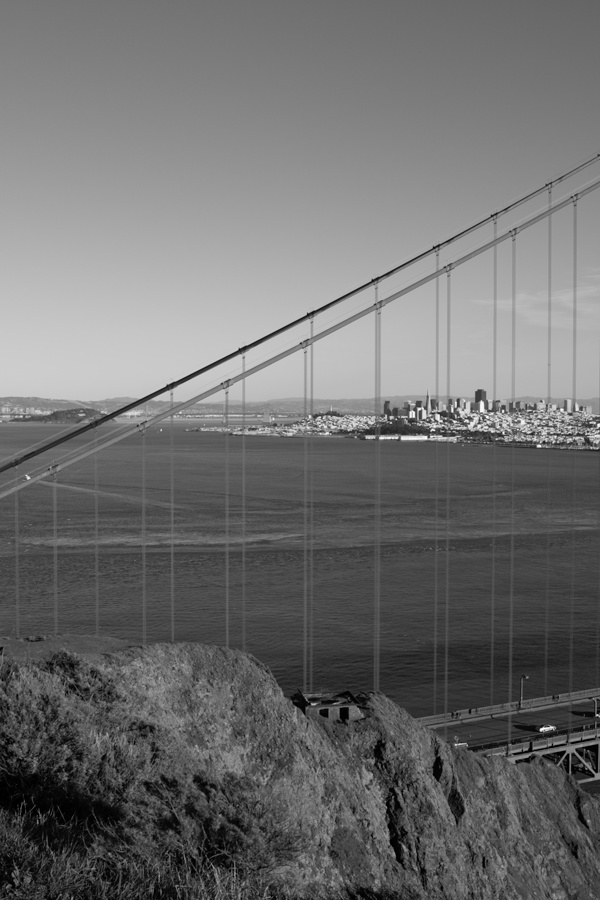
\includegraphics[width=0.16\textwidth]{../data/goldengate/01.jpg}
    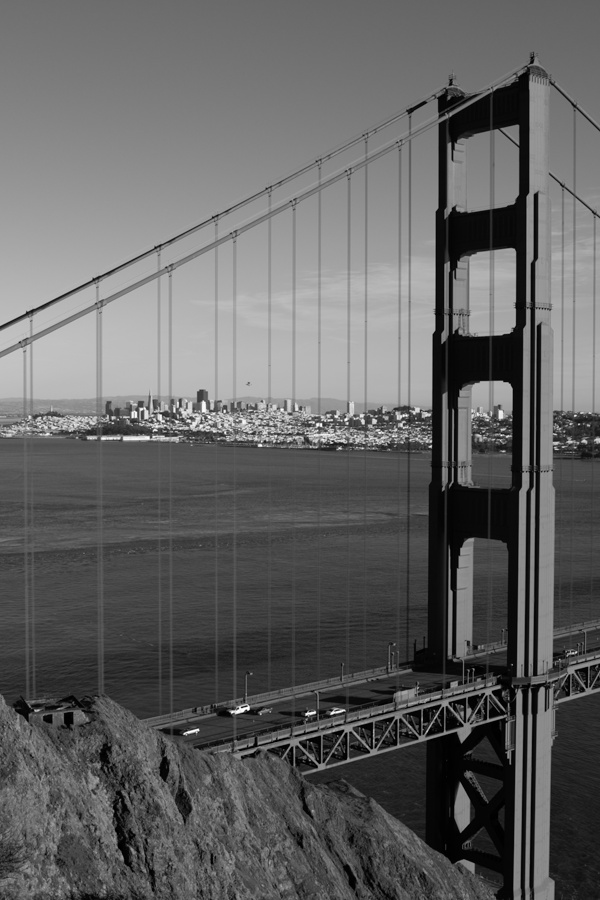
\includegraphics[width=0.16\textwidth]{../data/goldengate/02.jpg}
    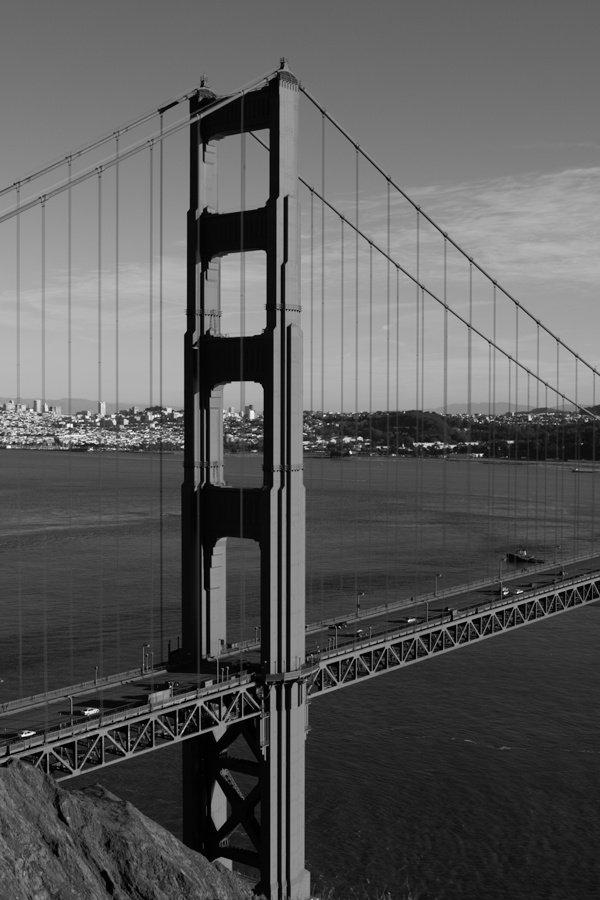
\includegraphics[width=0.16\textwidth]{../data/goldengate/03.jpg}
    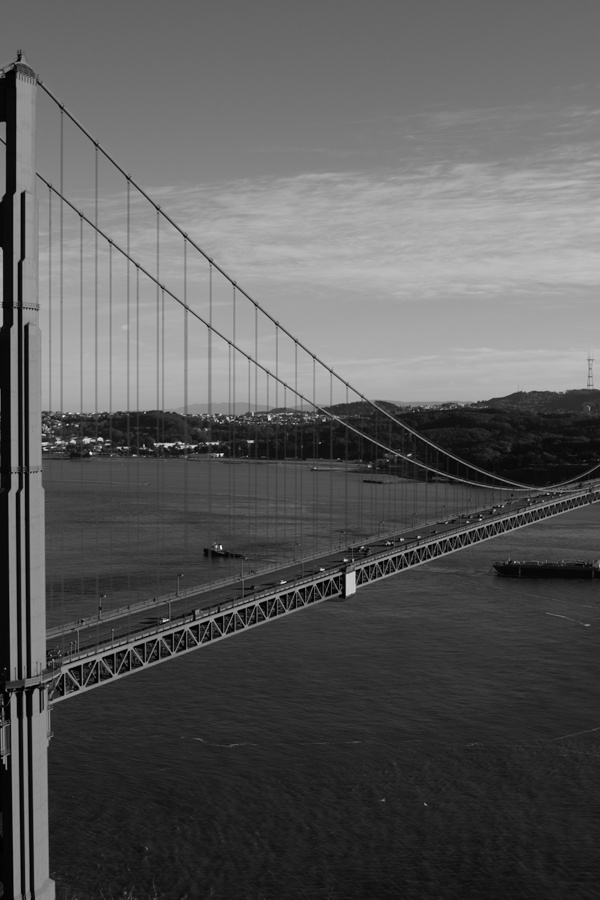
\includegraphics[width=0.16\textwidth]{../data/goldengate/04.jpg}
    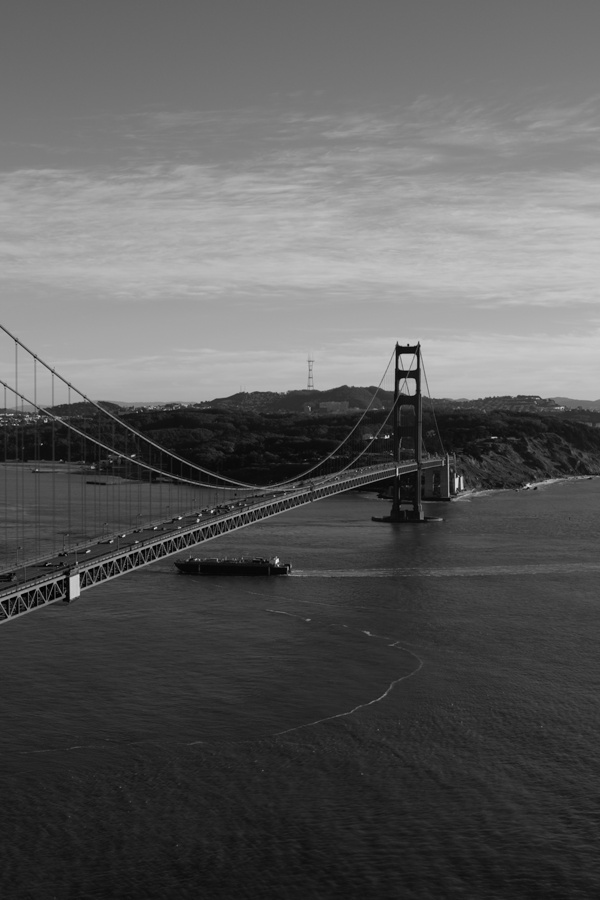
\includegraphics[width=0.16\textwidth]{../data/goldengate/05.jpg}
    \caption{原始照片}
    \label{fig:golden_org}
\end{figure}

\begin{figure}[H]
    \centering
    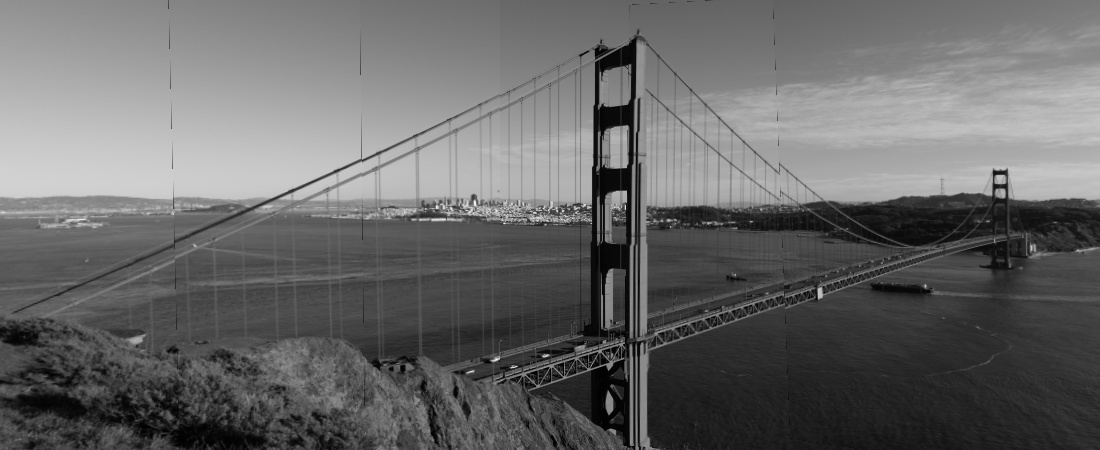
\includegraphics[width=1.0\textwidth]{../output/golden_paste.jpg}
    \caption{对齐后(直接叠加效果)}
    \label{fig:golden_align}
\end{figure}

\begin{figure}[H]
    \centering
    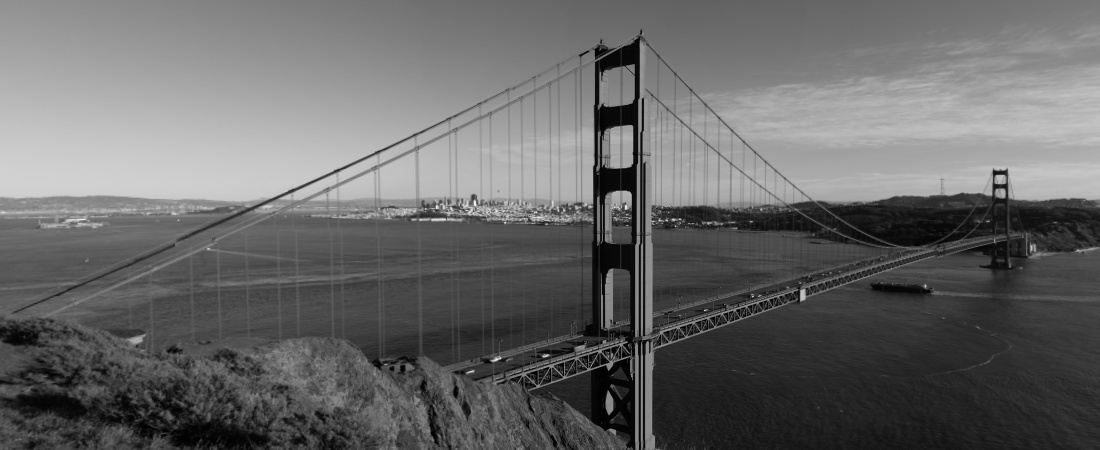
\includegraphics[width=1.0\textwidth]{../output/golden_poisson.jpg}
    \caption{GraphCut和泊松融合后最终效果}
    \label{fig:golden_poisson}
\end{figure}

\bibliographystyle{plain}
\bibliography{report}

\end{document}
